\documentclass[12pt,a4paper,twoside,openright,titlepage,final]{article}
\usepackage{fontspec}
\usepackage{amsmath}
\usepackage{amsfonts}
\usepackage{amssymb}
\usepackage{makeidx}
\usepackage{graphicx}
\usepackage[hidelinks,unicode=true]{hyperref}
\usepackage[spanish,es-nodecimaldot,es-lcroman,es-tabla,es-noshorthands]{babel}
\usepackage[left=3cm,right=2cm, bottom=4cm]{geometry}
\usepackage{natbib} 
\usepackage{microtype}
\usepackage{ifdraft}
\usepackage{verbatim}
\usepackage[obeyDraft]{todonotes}
\ifdraft{
	\usepackage{draftwatermark}
	\SetWatermarkText{BORRADOR}
	\SetWatermarkScale{0.7}
	\SetWatermarkColor{red}
}{}
\usepackage{booktabs}
\usepackage{longtable}
\usepackage{calc}
\usepackage{array}
\usepackage{caption}
\usepackage{subfigure}
\usepackage{footnote}
\usepackage{url}
\usepackage{tikz}

%\setsansfont[Ligatures=TeX]{texgyreadventor}
%\setmainfont[Ligatures=TeX]{texgyrepagella}

%*******************************************************
%                 NO MODIFICAR
\newcommand*{\FSfont}[1]{%
  \fontencoding{T1}\fontfamily{#1}\selectfont}

\newlength{\tpheight}\setlength{\tpheight}{0.9\textheight}
\newlength{\txtheight}\setlength{\txtheight}{0.9\tpheight}
\newlength{\tpwidth}\setlength{\tpwidth}{0.9\textwidth}
\newlength{\txtwidth}\setlength{\txtwidth}{0.9\tpwidth}
\newlength{\drop}
%*******************************************************

% Crea una portada con los siguientes parámetros
%
% #1 : Título 
% #2 : Subtítulo
% #3 : Subsubtítulo
% #4 : Autor(es)
% #5 : Lugar
%

\newcommand*{\portada}[5]{
\begin{titlepage}
\begingroup
\vspace*{1cm}
\drop = 0.2\txtheight
\centering
\vfill
{\Huge \scshape #1}\\[\baselineskip]
{\Large \textbf{#2}}\\[\baselineskip]
{\Large \scshape #3}\\[\baselineskip]
\vspace*{0.3cm}
{\large \textit{#4}}\\[0.5\drop]

\includegraphics[scale=0.35]{./imagenes/logoURJC.jpg}
\vspace*{1.5cm}

{\large \scshape #5, \today} \par
\begin{center}
\end{center}
\vfill\null
\endgroup
\end{titlepage}
}
 %*****************************************************
 


\author{José Ignacio Escribano}

\title{Práctica final}

\setlength{\parindent}{0pt}

\begin{document}

\pagenumbering{alph}
\setcounter{page}{1}

\portada{Práctica final}{Ingeniería de la Decisión}{Ruta óptima para llegar al trabajo}{José Ignacio Escribano}{Móstoles}

\listoffigures
\thispagestyle{empty}
\newpage

\tableofcontents
\thispagestyle{empty}
\newpage


\pagenumbering{arabic}
\setcounter{page}{1}

\section{Introducción}

Habitualmente, nos desplazamos para llegar al trabajo, y tenemos, en general, varias formas de ellas hasta él. Los medios de transporte disponibles son el coche, metro, autobús y Cercanías Renfe. Nuestro objetivo es llegar lo más rápido posible, es decir, minimizar el tiempo de llegada hasta el trabajo. Supondremos que nuestro trabajo se encuentra en la ciudad de Madrid, y hasta él tenemos una distancia de 30 kilómetros (por carretera). Preferimos los medios terrestres (coche y autobús) sobre los medios subterráneos (metro y Cercanías). Además de llegar lo antes posible, también queremos tener la máxima comodidad, que sea lo más barato y que contamine lo menos posible. Si se elige los servicios de transporte (metro, autobús o Cercanías) se quiere minimizar el número de transbordos.\\

\section{Resolución del problema}

\subsection{Estructuración del problema}

Para resolver el problema comenzamos identificando los distintos elementos que componen el problema, esto es, identificamos los factores de incertidumbre, los objetivos conflictivos, la influencia del tiempo, los decisores y los grupos afectados:\\

\begin{itemize}
	
	\item \textbf{Factores de incertidumbre}
	
	\begin{itemize}
		\item Condiciones meteorológicas (lluvia, nieve, hielo, sol, ...), precio del combustible, precio de los servicios de transporte, nivel de contaminación, la predicción meteorológica
	\end{itemize}
	
	\item \textbf{Objetivos conflictivos}
	
	\begin{itemize}
		\item Minimizar el tiempo de llegada, minimizar el coste, maximizar la comodidad, preferencia de medios terrestres sobre medios subterráneos, minimizar el número de transbordos, minimizar las emisiones de NO2.
	\end{itemize}
	
	\item \textbf{Influencia del tiempo}
	
	\begin{itemize}
		\item Condiciones meteorológicas, precio del combustible, precio de los servicios de transporte (tanto a corto como a largo plazo), día y hora en la que nos encontremos (por ejemplo, no es lo mismo ir a trabajar un domingo que habrá menos tráfico por la carretera, que un lunes por la mañana que seguramente habrá retenciones), apertura de nuevas carreteras o nuevos servicios en los medios de transporte.
	\end{itemize}
	
	\item \textbf{Decisores}
	
	\begin{itemize}
		\item Nosotros mismos
	\end{itemize}
	
	\item \textbf{Grupos afectados}
	
	\begin{itemize}
		\item Nosotros mismos, usuarios de los servicios de transporte, usuarios de coches, ciudadanos de Madrid (por la contaminación)
	\end{itemize}
\end{itemize}

Una vez que tenemos identificamos los elementos del problema, procedemos a crear el diagrama de influencia.\\

En primer lugar, ponemos las incertidumbres, los objetivos y las decisiones (elegir medio de transporte) en GeNIe (Figura~\ref{fig:diagrama_1}).\\
 

\begin{figure}[tbph!]
\centering
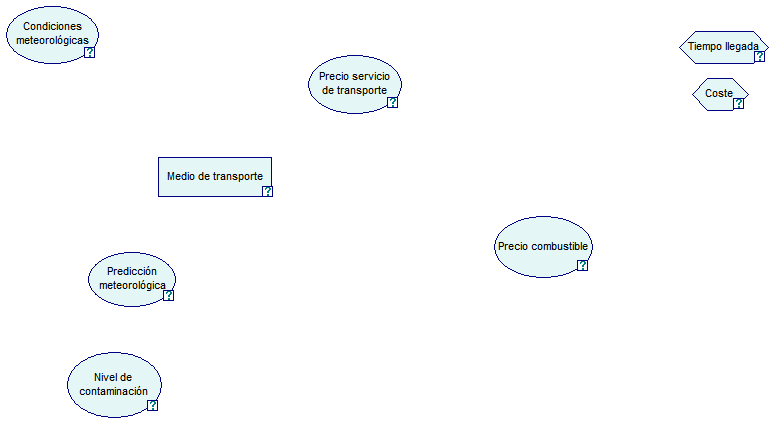
\includegraphics[width=0.9\linewidth]{imagenes/diagrama_1}
\caption{Primer boceto del diagrama de influencia}
\label{fig:diagrama_1}
\end{figure}

En este primer boceto, sólo introducimos los objetivos de minimizar el coste y el tiempo de llegada. Más adelante consideraremos los demás objetivos.\\

Nos queda introducir los arcos entre los nodos. Para ello, consideramos las influencias entre cada uno de los nodos (Figura~\ref{fig:diagrama_2}).\\

Comencemos con el nodo de Condiciones meteorológicas: hay un arco entre este nodo y nivel de contaminación ya que las condiciones meteorológicas condicionan el nivel de contaminación. También hay un arco hacia el nodo de valor Tiempo llegada ya que la meteorología influye en el tiempo que tardaremos en llegar al trabajo.\\

En el nodo Predicción meteorológica, tenemos un arco hacia Condiciones meteorológicas, ya que la condiciones meteorológica vendrán determinadas por las condiciones meteorológicas.\\

El precio del combustible condiciona al Precio del servicio de transporte, y ambos precios afectan al objetivo del coste.\\

Para tomar la decisión, conocemos la predicción meteorológica, las condiciones meteorológicas actuales, los precios del combustible y de los servicios de transporte, y el nivel de contaminación.

\begin{figure}[tbph!]
	\centering
	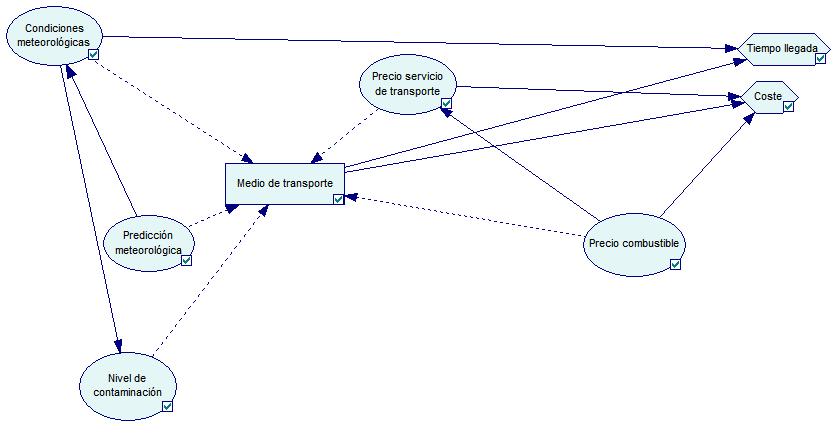
\includegraphics[width=0.9\linewidth]{imagenes/diagrama_2}
	\caption{Diagrama de influencia con los arcos}
	\label{fig:diagrama_2}
\end{figure}

\subsection{Modelización de creencias}

Ahora procedemos a asignar probabilidades a los nodos de azar.\\

En primer lugar consideraremos los estados de los nodos Condiciones y Predicción meteorológica. Éstos serán cuatro posibles: Lluvia, nieve, niebla y despejado.\\

Se sabe que la predicción de lluvia se dio el 15\% de los casos, nieve en el 5\%, niebla en el 10\% y despejado el 70\%. En la Figura~\ref{fig:prob_pred_met} se puede ver cómo queda en GeNIe.\\   

\begin{figure}[tbph!]
	\centering
	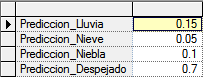
\includegraphics[width=0.3\linewidth]{imagenes/prob_pred_met}
	\caption{Estados y probabilidades del nodo Predicción meteorológica}
	\label{fig:prob_pred_met}
\end{figure}

También se conocen las probabilidades de que se produzcan las condiciones meteorológicas actuales dadas las predicción (Tabla~\ref{tbl:condicionadas}).

\begin{table}[htbp!]
	\centering
	\caption{Probabilidades de las condiciones condicionadas a las predicciones meteorológicas}
	\label{tbl:condicionadas}
	\begin{tabular}{@{}ccccc@{}}
		\toprule
		Condiciones\textbackslash Predicción & Lluvia & Nieve & Niebla & Despejado \\ \midrule
		Lluvia                               & 0.8    & 0.3   & 0.3    & 0.1       \\
		Nieve                                & 0.01   & 0.6   & 0.2    & 0.01      \\
		Niebla                               & 0.1    & 0.05  & 0.4    & 0.01      \\
		Despejado                            & 0.09   & 0.05  & 0.1    & 0.88      \\ \bottomrule
	\end{tabular}
\end{table} 

En el nodo Precio combustible consideramos dos estados: precio alto y bajo. Diremos que el precio es alto si nos cuesta 1 litro de gasolina más de 1.20 euros. En caso contrario, tenemos un precio bajo.\\

Se conoce que el 70\% de los días de los últimos cinco años, el precio del combustible ha estado alto. El 30\% ha estado bajo.\\

Con el precio del transporte tenemos, de nuevo, dos estados: precio alto y bajo. Consideraremos que el precio del transporte es alto si la media aritmética de los transportes públicos (metro, autobús y Cercanías) es mayor a 3 euros. En caso contrario, el precio es bajo.\\

Se saben las probabilidades del precio del transporte público, dado el precio del combustible (Tabla~\ref{tbl:condicionadas_2}).

\begin{table}[htbp!]
	\centering
	\caption{Probabilidades del precio del transporte condicionadas al precio del combustible}
	\label{tbl:condicionadas_2}
	\begin{tabular}{@{}ccc@{}}
		\toprule
		Precio transporte \textbackslash Precio combustible & Precio alto & Precio bajo \\ \midrule
		Precio alto                                         & 0.75        & 0.5         \\
		Precio bajo                                         & 0.25        & 0.5         \\ \bottomrule
	\end{tabular}
\end{table}

El último nodo que nos queda es el Nivel de contaminación. Tenemos dos estados contaminación alta y baja. Consideramos que el nivel es alto si se tiene una medida superior a 40 $\mu g/m^3$ anuales, y bajo en caso contrario.

Por último, conocemos la probabilidad del nivel de contaminación dadas las condiciones meteorológicas (Tabla~\ref{tbl:condicionadas_3}).

\begin{table}[htbp!]
	\centering
	\caption{Probabilidades del nivel de contaminación dadas las condiciones meteorológicas}
	\label{tbl:condicionadas_3}
	\begin{tabular}{@{}ccccc@{}}
		\toprule
		Nivel contaminación \textbackslash Condiciones meteorológicas & Lluvia & Nieve & Niebla & Despejado \\ \midrule
		Nivel alto                                                    & 0.7    & 0.5   & 0.4    & 0.3       \\
		Nivel bajo                                                    & 0.25   & 0.5   & 0.6    & 0.7       \\ \bottomrule
	\end{tabular}
\end{table}

Todos las probabilidades anteriores las introducimos en el modelo de GeNIe.

\subsection{Modelización de preferencias}

\subsection{Optimización}

\subsection{Análisis del modelo}

\section{Conclusiones}



\end{document} 